\subsubsection{Gripper for debris}
For rotating brush it was decided use DC motor. It allow the fastest collecting debris. \newline
The first part of module is the mount to the base and axis. The brush is fixed on it.
	\begin{center}
		\begin{tabular}{|p{0.14\linewidth}|p{0.12\linewidth}|p{0.12\linewidth}|}
			{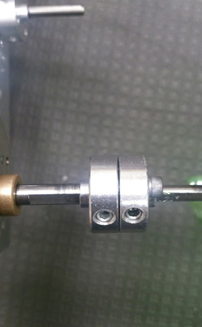
\includegraphics[scale=0.5]{days_L/Gripper/images/01}} & {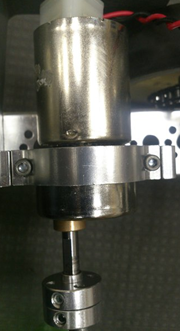
\includegraphics[scale=0.5]{days_L/Gripper/images/02}} & {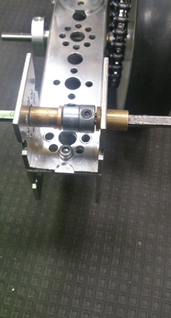
\includegraphics[scale=0.5]{days_L/Gripper/images/03}}\\
			\hline & Mount for axis  &
		\end{tabular}
	\end{center}
	Also it was made protection for wiring of the motor. It is the construction of Tetrix plates that fixed to the base rigidly.
\begin{figure}[H]
		\begin{minipage}[h]{\linewidth}
			\center{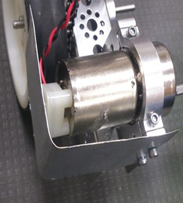
\includegraphics[scale=0.5]{days_L/Gripper/images/04}}
			\caption{Protection on DCmotor}
		\end{minipage}
	\end{figure}
	The next element of the module is the brush. The brush should be tough enough so that it doesn't bend during collecting debris. But it should be elastic in order to when robot hit the wall of field the brush bend but not broke.\newline
	At first it was made brush made of piece of plastic bottle. During the test it collect debris good enough but it started crack.
	\begin{figure}[H]
		\begin{minipage}[h]{1\linewidth}
			\center{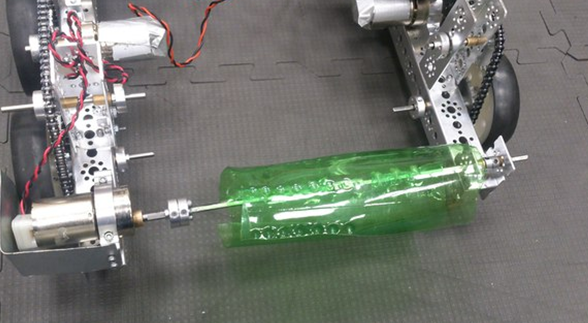
\includegraphics[scale=0.5]{days_L/Gripper/images/05}}
			\caption{Brush madde of plastic bottle}
		\end{minipage}
	\end{figure}
	So it was decided to use pieces of rubber hose because it is elastic but more durable than plastic. Pieces of hose were fixed on the aluminium tube from Tetrix set with help of screws. The tube was instaled on the shaft of motor instead of axis. This construction worked good enough. It collected debris without problems.  
	\begin{figure}[H]
		\begin{minipage}[h]{\linewidth}
			\center{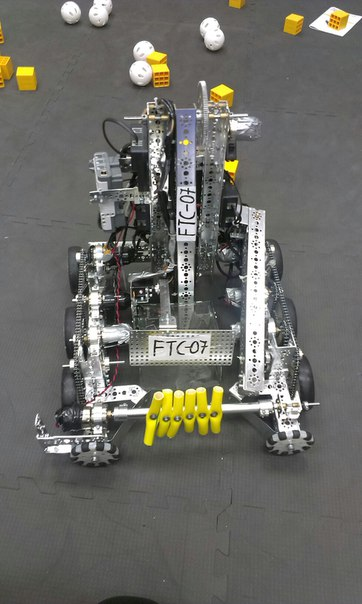
\includegraphics[scale=0.5]{days_L/Gripper/images/06}}
			\caption{Gripper with hose}
		\end{minipage}
	\end{figure}
	Later it was decided to increace speed of rotation gripper and install transmission with gear ratio 2:1. It need for pushing away scoring elements durin autonomous period.
   \begin{figure}[H]
		\begin{minipage}[h]{\linewidth}
			\center{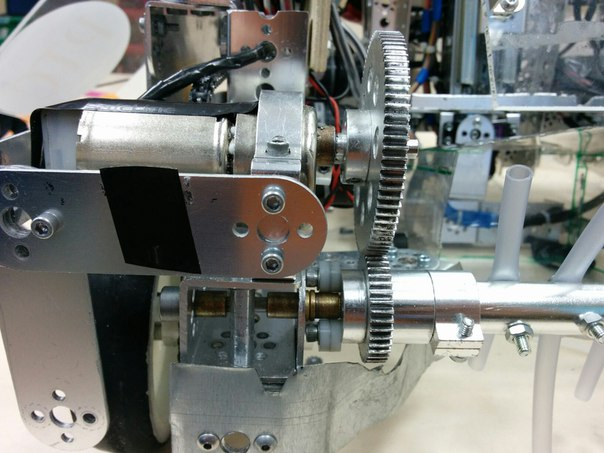
\includegraphics[scale=0.5]{days_L/Gripper/images/07}}
			\caption{Transmission with gear}
		\end{minipage}
	\end{figure}   
But this construction doesn't worked, because Pieces of hose were inflexible and rested in scoring elements while robot doesn't moved. So we decided to use tubes from a dropper. Also we can add more tubes, because they not so wide. This construction worked very well.
   \begin{figure}[H]
		\begin{minipage}[h]{\linewidth}
			\center{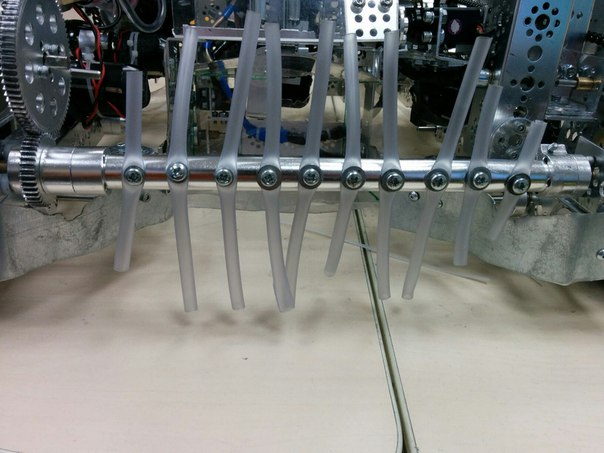
\includegraphics[scale=0.5]{days_L/Gripper/images/08}}
			\caption{Gripper with tubes from dropper}
		\end{minipage}
	\end{figure}
	
\fillpage	
